\documentclass[aspectratio=169]{beamer}
\usepackage{pgf}
\usepackage{colortbl,tabularx,mathrsfs,calligra}
\usepackage{amsmath,amsfonts,amssymb,amsthm}
\usepackage{ragged2e}
\usepackage{setspace}
\usepackage{filecontents}
\usepackage{caption}
\usepackage{subcaption}
\usepackage{contour}
\usepackage{fancybox}
\usepackage{wrapfig}
\usepackage{multirow}
\usepackage{multicol}
\usepackage{tikz, pgfplots, tkz-euclide,calc}
    \usetikzlibrary{patterns,snakes,shapes.arrows}
\usepackage{listings}
\usepackage{enumitem}
\usepackage{pifont}
% \usepackage[scaled]{berasans}
%     \renewcommand*\familydefault{\sfdefault}  %% Only if the base font of the document is to be sans serif
% \usepackage[T1]{fontenc}
\usepackage[scaled]{uarial}
\renewcommand*\familydefault{\sfdefault} %% Only if the base font of the document is to be sans serif
\usepackage[T1]{fontenc}

\graphicspath{{C:/Users/teoso/OneDrive/Documents/Asisten Dosen & Lab/Asisten Dosen/PPT Kalkulus/Gambar & Logo/}}

\definecolor{HIMAmuda}{HTML}{01D1FD}
\definecolor{HIMAtua}{HTML}{02016A}
\definecolor{HIMAabu}{HTML}{CBCBCC}
\definecolor{PastelGreen}{HTML}{77DD77}

\usetheme{Madrid}

\setbeamercolor{palette primary}{bg=HIMAtua,fg=white}
\setbeamercolor{palette secondary}{bg=HIMAmuda,fg=black}
\setbeamercolor{palette tertiary}{bg=HIMAabu,fg=black}
\setbeamercolor{palette quaternary}{bg=HIMAmuda,fg=white}
\setbeamercolor{structure}{fg=HIMAmuda} % itemize, enumerate, etc
\setbeamercolor{section in toc}{fg=HIMAtua} % TOC sections
\setbeamercolor{block title alerted}{fg=white,bg=magenta}
\setbeamercolor{block body alerted}{fg=black!90,bg=pink}

\usefonttheme{professionalfonts}
\setbeamertemplate{theorems}[numbered]
\setbeamertemplate{itemize items}[circle]

\usebackgroundtemplate{%
\tikz[overlay,remember picture] \node[opacity=0.1, at=(current page.center)]{
\includegraphics[width=\paperwidth]{arona class}};
}

\renewcommand\thesubfigure{\arabic{subfigure}}
\newtheorem*{funfact}{Fun Fact}
\newtheorem{latihan}{Latihan}
\newtheorem{definisi}{Definisi}
\newtheorem{teorema}{Teorema}
\theoremstyle{definition}
\newtheorem*{contoh}{Contoh}
\newcommand{\R}{\mathbb{R}}

\AtBeginEnvironment{funfact}{%
  \setbeamercolor{block title}{fg=white,bg=PastelGreen} % Set title background to pastel green and text to white
  \setbeamercolor{block body}{parent=normal text,bg=PastelGreen!30!white} % Set body background to a lighter pastel green
}
\AtBeginEnvironment{definisi}{
    \setbeamercolor{block title}{fg=white,bg=HIMAtua}
    \setbeamercolor{block body}{parent=normal text,bg=HIMAtua!30!white}
}
\AtBeginEnvironment{teorema}{
    \setbeamercolor{block title}{bg=darkgray,fg=white}
    \setbeamercolor{block body}{parent=pallette tertiary,bg=HIMAabu!30!white}
}


\author[Tetew]{Teosofi Hidayah Agung}
\date{5 September 2024}
\title[Kalkulus 1 - Bab 1]{Sistem Bilangan Real}
\institute[Matematika ITS]{Departemen Matematika\\ Institut Teknologi Sepuluh Nopember}
\titlegraphic{{
\includegraphics[scale=0.3]{ITS.png}$\quad$
\includegraphics[scale=0.02]{M.png}}}

\begin{document}
    {\usebackgroundtemplate{
        \tikz[overlay,remember picture] \node[opacity=0.1, at=(current page.center)]{
\includegraphics[width=\paperwidth]{yuuka s}};}
    \begin{frame}
        \titlepage
    \end{frame}
    }

    \begin{frame}{Daftar isi}
        \tableofcontents
    \end{frame}

    \section{Bilangan Real}

    {\usebackgroundtemplate{
        \tikz[overlay,remember picture] \node[opacity=0.2, at=(current page.center)]{
\includegraphics[width=\paperwidth]{motivated.jpg}};
        }
    \begin{frame}
        \frametitle{\insertsection}
        \begin{block}{Motivasi}
            \begin{itemize}
                \item[\ding{51}] Berapa banyak bilangan bulat antara 1 dan 10?
                \item[\ding{51}] Berapa banyak bilangan bulat dari 0 sampai 1?
                \item[\ding{51}] Berapa banyak bilangan real yang berada antara 0 dan 1? 
            \end{itemize}      
        \end{block}
        \onslide<2->\begin{funfact}
            Pernyataan $1=0,999\ldots$ adalah benar.
        \end{funfact}
    \end{frame}
    }

    \begin{frame}
        \frametitle{\insertsection}
        \begin{definisi}
            Bilangan real adalah himpunan yang mencakup semua bilangan yang dapat ditemukan pada garis bilangan, termasuk bilangan bulat, bilangan pecahan, dan bilangan irasional. Bilangan real biasanya dilambangkan dengan simbol $\R$.
        \end{definisi}
        \onslide<2->{Himpunan bagian dari $\R$ sering dinyatakan dalam bentuk interval
        \[(a,b]=\{x\,|\,a<x\leq b\}\]
        dan dapat digambarkan dalam garis bilangan
        \begin{center}
            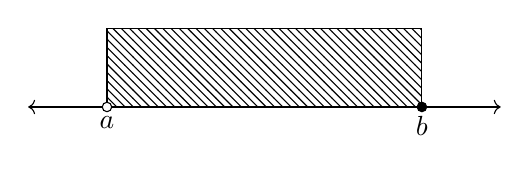
\begin{tikzpicture}
                \draw[<->] (-1,0) -- (5,0);
                \draw[pattern=north west lines] (0,0) -- (4,0)--(4,1)--(0,1)--cycle;
                \draw[fill=white] (0,0) circle (0.06) node[below]{$a$};
                \draw[fill=black] (4,0) circle (0.06) node[below]{$b$};
            \end{tikzpicture}
        \end{center}}
    \end{frame}

    \begin{frame}
        \frametitle{\insertsection}
        \begin{alertblock}{Peringatan}
            Konsep "pindah ruas" sebenarnya tidak ada.
        \end{alertblock}
        \onslide<2->\begin{teorema}
            Diberikan bilangan real $a,b,$ dan $c$:
            \begin{enumerate}[label=(\roman*)]
                \item Jika $a<b$, maka $a\pm c<b\pm c$.
                \item Jika $a<b$ dan $c>0$, maka $ac<bc$ dan $a/c<b/c$.
                \item Jika $a<b$ dan $c<0$, maka $ac>bc$ dan $a/c>b/c$.
                \item Jika $a<b$ dan keduanya positif atau keduanya negatif, maka $\displaystyle\frac{1}{b}<\frac{1}{a}$.
            \end{enumerate}
        \end{teorema}
    \end{frame}

    \begin{frame}
        \frametitle{\insertsection}
        Misalkan $p<q=r<s$, maka $[p,q)\cup[r,s]$ dapat diilustrasikan sebagai berikut
        \begin{center}
            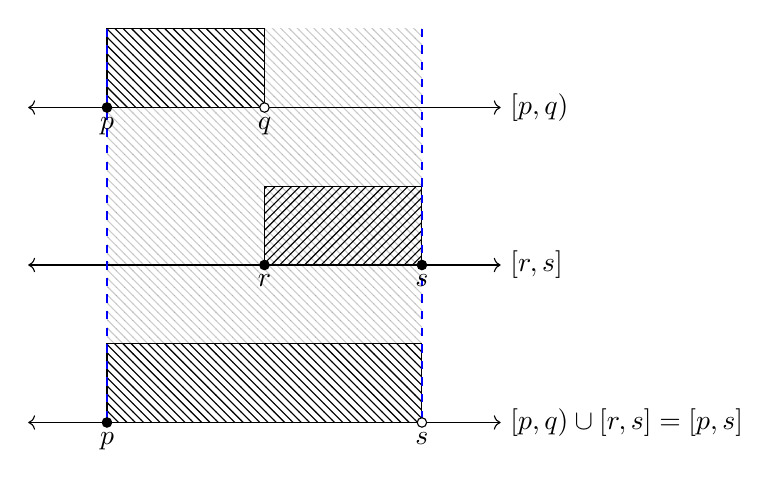
\begin{tikzpicture}
                \draw[<->] (-1,0) -- (5,0) node[right]{$[r,s]$};
                \draw[<->] (-1,2) -- (5,2) node[right]{$[p,q)$};
                \draw[<->] (-1,-2) -- (5,-2) node[right]{$[p,q)\cup[r,s]=[p,s]$};
                
                \draw[pattern=north west lines] (0,2) -- (2,2)--(2,3)--(0,3)--cycle;
                \draw[pattern=north east lines] (2,0) -- (4,0)--(4,1)--(2,1)--cycle;
                \draw[pattern=north west lines] (0,-2) -- (4,-2)--(4,-1)--(0,-1)--cycle;

                \draw[thick,dashed,blue] (0,3) -- (0,-2);
                \draw[thick,dashed,blue] (4,3) -- (4,-2);
                \fill[pattern=north west lines,opacity=0.2] (0,3) rectangle (4,-2);

                \draw[fill=black] (0,2) circle (0.06) node[below]{$p$};
                \draw[fill=white] (2,2) circle (0.06) node[below]{$q$};
                \draw[fill=black] (2,0) circle (0.06) node[below]{$r$};
                \draw[fill=black] (4,0) circle (0.06) node[below]{$s$};
                \draw[fill=white] (4,-2) circle (0.06) node[below]{$s$};
                \draw[fill=black] (0,-2) circle (0.06) node[below]{$p$};
            \end{tikzpicture}
        \end{center}
    \end{frame}

    \begin{frame}
        \frametitle{\insertsection}
        Misalkan $a<c<b<d$, maka $[a,b)\cap[c,d]$ dapat diilustrasikan sebagai berikut
        \begin{center}
            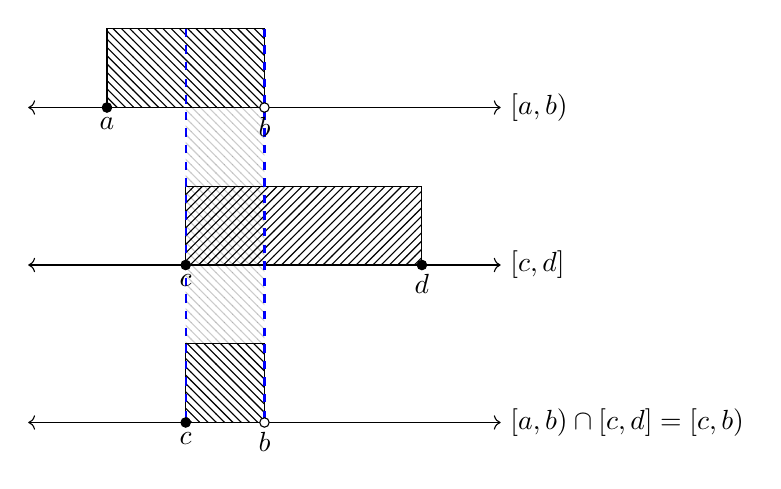
\begin{tikzpicture}
                \draw[<->] (-1,0) -- (5,0) node[right]{$[c,d]$};
                \draw[<->] (-1,2) -- (5,2) node[right]{$[a,b)$};
                \draw[<->] (-1,-2) -- (5,-2) node[right]{$[a,b)\cap[c,d]=[c,b)$};
                
                \draw[pattern=north west lines] (0,2) -- (2,2)--(2,3)--(0,3)--cycle;
                \draw[pattern=north east lines] (1,0) -- (4,0)--(4,1)--(1,1)--cycle;
                \draw[pattern=north west lines] (1,-2) -- (2,-2)--(2,-1)--(1,-1)--cycle;

                \draw[thick,dashed,blue] (1,3) -- (1,-2);
                \draw[thick,dashed,blue] (2,3) -- (2,-2);
                \fill[pattern=north west lines,opacity=0.2] (1,3) rectangle (2,-2);

                \draw[fill=black] (0,2) circle (0.06) node[below]{$a$};
                \draw[fill=white] (2,2) circle (0.06) node[below]{$b$};
                \draw[fill=black] (1,0) circle (0.06) node[below]{$c$};
                \draw[fill=black] (4,0) circle (0.06) node[below]{$d$};
                \draw[fill=white] (2,-2) circle (0.06) node[below]{$b$};
                \draw[fill=black] (1,-2) circle (0.06) node[below]{$c$};
            \end{tikzpicture}
        \end{center}
    \end{frame}

    \begin{frame}
        \frametitle{\insertsection}
        \begin{exampleblock}{Latihan}
            Tentukan nilai dari $x$ yang memenuhi pertidaksamaan berikut
            \begin{enumerate}[label=(\alph*)]
                \item $2\leq x^2+x<12$.
                \item $x^3-4x^2-15x+18>0$.
                \item $\displaystyle\frac{2x}{x-4}\geq\frac{1}{x-3}$.
            \end{enumerate}
        \end{exampleblock}
    \end{frame}

    \section{Nilai Mutlak}
    \begin{frame}
        \frametitle{\insertsection}
        \begin{definisi}
            Nilai mutlak dari bilangan real $x$ adalah
            \[|x|=\begin{cases}
                x & \text{jika } x\geq 0,\\
                -x & \text{jika } x<0.
            \end{cases}\]
        \end{definisi}
        \onslide<2->\begin{teorema}
            Misalkan $a$ dan $b$ adalah bilangan real, maka jarak antara $a$ dan $b$ adalah $d=|a-b|$. Dalam pertidaksamaan, solusinya dapat dinyatakan sebagai berikut\\
            \begin{center}
            \begin{tabular}{c|c|c}
                \hline
                Pertidaksamaan &Bentuk lain& Solusi\\
                \hline
                $|x-a|<b$ &$-b<x-a<b$& $a-b<x<a+b$\\
                $|x-a|>b$ &$x-a<-b$ atau $x-a>b$& $x<a-b \text{ atau } x>a+b$\\
            \end{tabular}
        \end{center}
        \end{teorema}
    \end{frame}

    \begin{frame}
        \frametitle{\insertsection}
        \begin{exampleblock}{Latihan}
            Tentukan solusi dari pertidaksamaan berikut
            \begin{enumerate}[label=(\alph*)]
                \item $|x-2|<3$.
                \item $2<|x-1|<5$.
                \item $|x+1|+|x-2|<4$.
            \end{enumerate}
        \end{exampleblock}
    \end{frame}

    \section{Grafik Persamaan}
    \begin{frame}
        \frametitle{\insertsection}
        Grafik-grafik dasar
        \begin{center}
            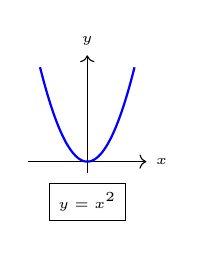
\begin{tikzpicture}[scale=0.3]
                % Gambar sumbu x dan y
                \draw[->] (-2.5,0) -- (2.5,0) node[right] {\tiny$x$};
                \draw[->] (0,-0.5) node[below] {\tiny$\boxed{y=x^2}$} -- (0,4.5) node[above] {\tiny$y$};

                \draw[thick, domain=-2:2, samples=100,blue] plot (\x, {(\x)^2});
            \end{tikzpicture}
            $\quad$
            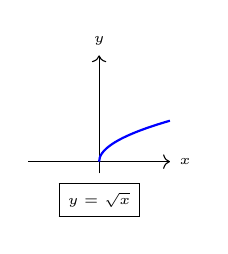
\begin{tikzpicture}[scale=0.3]
                % Gambar sumbu x dan y
                \draw[->] (-3,0) -- (3,0) node[right] {\tiny$x$};
                \draw[->] (0,-0.5) node[below] {\tiny$\boxed{y=\sqrt{x}}$} -- (0,4.5) node[above] {\tiny$y$};

                \draw[thick, domain=0:3, samples=100,blue] plot (\x, {sqrt(\x)});
            \end{tikzpicture}
            $\quad$
            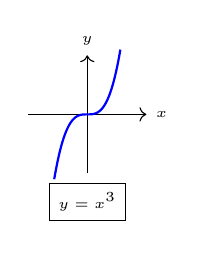
\begin{tikzpicture}[scale=0.3]
                % Gambar sumbu x dan y
                \draw[->] (-2.5,0) -- (2.5,0) node[right] {\tiny$x$};
                \draw[->] (0,-2.5) node[below] {\tiny$\boxed{y=x^3}$} -- (0,2.5) node[above] {\tiny$y$};

                \draw[thick, domain=-1.4:1.4, samples=100,blue] plot (\x, {(\x)^3});
            \end{tikzpicture}
            $\quad$
            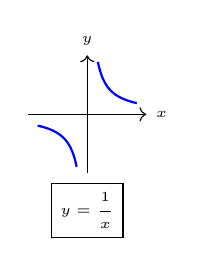
\begin{tikzpicture}[scale=0.3]
                % Gambar sumbu x dan y
                \draw[->] (-2.5,0) -- (2.5,0) node[right] {\tiny$x$};
                \draw[->] (0,-2.5) node[below] {\tiny$\displaystyle\boxed{y=\frac{1}{x}}$} -- (0,2.5) node[above] {\tiny$y$};

                \draw[thick, domain=0.45:2.1, samples=100,blue] plot (\x, {1/(\x)});
                \draw[thick, domain=-2.1:-0.45, samples=100,blue] plot (\x, {1/(\x)});
            \end{tikzpicture}
            $\quad$
            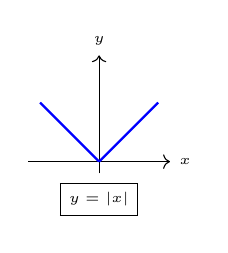
\begin{tikzpicture}[scale=0.3]
                % Gambar sumbu x dan y
                \draw[->] (-3,0) -- (3,0) node[right] {\tiny$x$};
                \draw[->] (0,-0.5) node[below] {\tiny$\boxed{y=|x|}$} -- (0,4.5) node[above] {\tiny$y$};

                \draw[thick, domain=-2.5:2.5, samples=100,blue] plot (\x, {abs(\x)});
            \end{tikzpicture}
        \end{center}
    \end{frame}

    \begin{frame}
        \frametitle{\insertsection}
        \begin{teorema}
            Misalkan $y=f(x)$ adalah fungsi dan $c>0$ adalah sebarang konstanta, maka pergeseran grafik $f(x)$ akan didapatkan hasil sebagai berikut 
            \begin{center}
                \begin{tabular}{c|c}
                    Persamaan Baru & Efek Geometri\\
                    \hline
                    $y=f(x)+c$ & Pergeseran $c$ satuan ke atas\\
                    $y=f(x)-c$ & Pergeseran $c$ satuan ke bawah\\
                    $y=f(x+c)$ & Pergeseran $c$ satuan ke kiri\\
                    $y=f(x-c)$ & Pergeseran $c$ satuan ke kanan\\
                \end{tabular}
            \end{center}
        \end{teorema}
    \end{frame}

    \begin{frame}
        \frametitle{\insertsection}
        \begin{exampleblock}{Latihan}
            Ilustrasikan grafik dari fungsi berikut:
            \begin{enumerate}[label=(\alph*)]
                \item $y=x^2+2$.
                \item $y=\displaystyle\frac{1}{x+1}-1$.
                \item $y=|x-2|+2$.
            \end{enumerate}
        \end{exampleblock}
    \end{frame}

    \section{Persamaan Garis dan Jarak}
    \begin{frame}
        \frametitle{\insertsection}
        \begin{definisi}
            Persamaan garis yang melalui dua titik $P(x_1,y_1)$ dan $Q(x_2,y_2)$ adalah
            \[y-y_1=\frac{y_2-y_1}{x_2-x_1}(x-x_1)\]
        \end{definisi}
        \begin{center}
            \begin{tikzpicture}
                \draw[-Latex] (-0.5,0) -- (3,0) node[right] {\tiny$x$};
                \draw[-Latex] (0,-0.5) -- (0,3) node[above] {\tiny$y$};
                \draw[fill=black] (0.5,0.5) circle (0.06) node[below right]{\tiny$P(x_1,y_1)$};
                \draw[fill=black] (3,2) circle (0.06) node[below right]{\tiny$Q(x_2,y_2)$};
                \draw[thick,blue] (0.5,0.5) -- (3,2);
                \draw[thick, domain=-1:3.5, samples=50,blue,dashed] plot (\x, {0.6*\x+0.2});
            \end{tikzpicture}
        \end{center}
    \end{frame}

    \begin{frame}
        \frametitle{\insertsection}
        \begin{teorema}
            Jarak antara dua titik $(x_1,y_1)$ dan $(x_2,y_2)$ adalah
            \[d=\sqrt{(x_2-x_1)^2+(y_2-y_1)^2}\] 
        \end{teorema}
        Dapat dibuktikan dengan menggunakan teorema Pythagoras
        \onslide<2->{\begin{teorema}
            Jarak antara titik $(x_1,y_1)$ dan garis $ax+by+c=0$ adalah
            \[d=\frac{|ax_1+by_1+c|}{\sqrt{a^2+b^2}}\]
        \end{teorema}
        Pembuktian ada pada buku halaman 27}
    \end{frame}

    \begin{frame}
        \frametitle{\insertsection}
        \begin{exampleblock}{Latihan}
            \begin{enumerate}[label=(\arabic*)]
                \item Tentukan jarak terdekat antara garis $y=2x+1$ dan garis $y=2x+5$.
                \item Diberikan $f(3)=7$ dan $f(5)=1$, tentukan persamaan garis yang melalui kedua titik tersebut.
                \item Carilah semua titik yang berjarak 5 dari titik $(1,2)$.
            \end{enumerate}
        \end{exampleblock}
    \end{frame}

    \section{Persamaan Lingkaran dan Parabola}
    \begin{frame}
        \frametitle{\insertsection}
        \begin{definisi}
            Persamaan lingkaran dengan pusat $(h,k)$ dan jari-jari $r$ adalah
            \[(x-h)^2+(y-k)^2=r^2\]
        \end{definisi}
        \begin{center}
            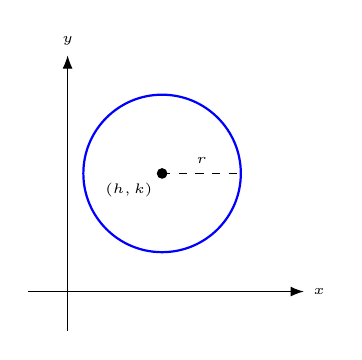
\begin{tikzpicture}
                \draw[-Latex] (-0.5,0) -- (3,0) node[right] {\tiny$x$};
                \draw[-Latex] (0,-0.5) -- (0,3) node[above] {\tiny$y$};
                \draw[fill=black] (1.2,1.5) circle (0.06) node[below left]{\tiny$(h,k)$};
                \draw[thick,blue] (1.2,1.5) circle (1);
                \draw[dashed] (1.2,1.5) -- node[above] {\tiny$r$} (2.2,1.5);
            \end{tikzpicture}
        \end{center}
    \end{frame}

    \begin{frame}
        \frametitle{\insertsection}
        \begin{definisi}
            Persamaan standar parabola dengan titik puncak $(h,k)$ dengan $a$ sebagai konstanta adalah
            \[y-k=a(x-h)^2\]
        \end{definisi}
        \begin{center}
            \begin{tikzpicture}
                \draw[-Latex] (-0.5,0) -- (3,0) node[right] {\tiny$x$};
                \draw[-Latex] (0,-0.5) -- (0,3) node[above] {\tiny$y$};
                \draw[fill=black] (1.5,0.5) circle (0.06) node[below left]{\tiny$(h,k)$};
                \draw[thick, domain=0.1:2.9, samples=50,blue] plot (\x, {(\x-1.5)^2+0.5});
            \end{tikzpicture}
        \end{center}
    \end{frame}

    \begin{frame}
        \frametitle{\insertsection}
        \begin{exampleblock}{Latihan}
            \begin{enumerate}[label=(\arabic*)]
                \item Gambarkan grafik $y=\sqrt{25-x^2}$.
                \item Apakah titik $(1,2)$ berada di dalam/pada/di luar lingkaran $x^2+y^2-6x-8y+9=0$? Berikan alasan anda.
                \item Tentukan persamaan parabola yang melalui titik $(1,2)$ dan $(3,4)$.
            \end{enumerate}
        \end{exampleblock}
    \end{frame}

    {
    \usebackgroundtemplate{
            \tikz[overlay,remember picture] \node[opacity=0.2, at=(current page.center)]{
\includegraphics[width=\paperwidth]{sudah saatnya}};
            }
    \setbeamercolor{block title}{bg=brown,fg=white} % Block title background brown, text white
    \setbeamercolor{block body}{bg=brown!30,fg=black}    
    \begin{frame}
        \begin{block}{\huge Quest}
            \huge Pilih 2 soal (terserah) dari soal latihan slide sebelumnya 
        \end{block}
    \end{frame}}
\end{document}